\documentclass{article}

\usepackage{graphicx}
\usepackage{setspace}
\usepackage{listings}
\usepackage{color}
\usepackage{circuitikz}
\usepackage{float}

\definecolor{dkgreen}{rgb}{0,0.6,0}
\definecolor{gray}{rgb}{0.5,0.5,0.5}
\definecolor{mauve}{rgb}{0.58,0,0.82}

\lstset{basicstyle=\small,
        keywordstyle=\color{mauve},
        identifierstyle=\color{dkgreen},
        stringstyle=\color{gray},
        numbers=left
        }

\title{ECE 210 - Combinational Logic Design \\ Lab 2}
\date{2018-10-24}
\author{David Lenfesty \\ lenfesty@ualberta.ca
    \and Radomir Wasowski \\ wasowski@ualberta.ca}

\setcounter{tocdepth}{2} % Show subsections

\begin{document}

    \doublespacing
    \pagenumbering{gobble}
    \maketitle
    \newpage

    \singlespacing
    \pagenumbering{arabic}

    \section{Abstract}

    It is often the case that more fundamental elements in any field can be
    combined to produce more complex and useful structures. This is certainly
    true in the field of circuit design, where discrete elements are used
    to create functional applications all the time.

    Multiplexers and demultiplexers can be used together to route specific
    incoming signals to a specified destination one at a time through a
    shared transmission line. The requirement of this lab was to design
    boolean expressions realizing the functionality of multiplexers and
    demultiplexers in the context of a real-life application.
    
    Another real-life application of logical elements is in an access control
    system. A simplistic version of such a system was also designed in this
    lab session and tested on an FPGA afterwards.

    \section{Introduction}

    The purpose of this lab was to design control circuits according to the provided
    specifications, and then verify their operation using a simulation or an FPGA.

    In the first part of the lab, a series of boolean expressions
    were designed to implement a Multiplexer/Demultiplexer circuit,
    intended to route data from one of three radio recievers to one
    of three engineers, and signal which engineer was currently
    recieving data.
    First, Xilinx Vivado Software was used to produce a circuit
    to fulfill this objective. Then, using the same software,
    the circuit was simulated against input combinations which
    would be encountered during normal use, for verification.

    For the second part of the lab, an Access Control circuit was to be designed,
    allowing lab entry only if a valid ID was provided alongside a proper keypad
    combination. Otherwise, an alarm signal was to be sent out.
    The method of designing this circuit was very similar to the method in part one:
    Again using Xilinx Vivado, the circuit was designed and simulated against inputs
    to verify if the outputs matched those in the specification.
    However, for this section, the design was also uploaded to a physical FPGA board
    where various could be manually tested and validated.

    \section{Design Section}

    In order to design the desired systems, the Xilinx Vivado software was
    used to write VHDL code that described the operation of each circuit.


    \newpage
    \paragraph{MUX / DEMUX Circuit}
    To implement the multiplexing/demultiplexing system, the following circuit had to be written in VHDL.

    \begin{circuitikz}[scale=0.75, transform shape]
        \draw
            % Input selection 0
            (0,0) node[american and port](IS0){}
            (2,-1) node[american and port](sig_in_0){}
            (IS0.in 1) node[anchor=east]{S0'}
            (IS0.in 2) node[anchor=east]{S1'}
            (IS0.out) -| (sig_in_0.in 1)
            (-2,-1) node[anchor=east, color=green]{I0} -| (sig_in_0.in 2)

            % Input selection 1
            (0,-2) node[american and port](IS1){}
            (2,-3) node[american and port](sig_in_1){}
            (IS1.in 1) node[anchor=east]{S0}
            (IS1.in 2) node[anchor=east]{S1'}
            (IS1.out) -| (sig_in_1.in 1)
            (-2,-3) node[anchor=east, color=green]{I1} -| (sig_in_1.in 2)

            % Input selection 2
            (0,-4) node[american and port](IS2){}
            (2,-5) node[american and port](sig_in_2){}
            (IS2.in 1) node[anchor=east]{S0}
            (IS2.in 2) node[anchor=east]{S1'}
            (IS2.out) -| (sig_in_2.in 1)
            (-2,-5) node[anchor=east, color=green]{I2} -| (sig_in_2.in 2)

            % OR accumulation for inputs
            (4,-2) node[american or port](mux_or_1){}
            (6,-3) node[american or port](mux_or_2){}
            (sig_in_0.out) -| (mux_or_1.in 1){}
            (sig_in_1.out) -| (mux_or_1.in 2){}
            (mux_or_1.out) -| (mux_or_2.in 1){}
            (sig_in_2.out) -| (mux_or_2.in 2){}

            % Engineer 0 selection
            (2,-8)  node[american and port](eng0_sel){}
            (4,-7)  node[american and port](eng0_sig){}
            (eng0_sel.in 1) node[anchor=east]{DS0'}
            (eng0_sel.in 2) node[anchor=east]{DS1'}
            (eng0_sel.out) -| (eng0_sig.in 2){}
            (eng0_sig.out) -| (7,-7) node[anchor=west, color=red]{E0}

            % Engineer 1 selection
            (2,-10) node[american and port](eng1_sel){}
            (4,-9)  node[american and port](eng1_sig){}
            (eng1_sel.in 1) node[anchor=east]{DS0'}
            (eng1_sel.in 2) node[anchor=east]{DS1'}
            (eng1_sel.out) -| (eng1_sig.in 2){}
            (eng1_sig.out) -| (7,-9) node[anchor=west, color=red]{E1}

            % Engineer 2 selection
            (2,-12) node[american and port](eng2_sel){}
            (4,-11) node[american and port](eng2_sig){}
            (eng2_sel.in 1) node[anchor=east]{DS0'}
            (eng2_sel.in 2) node[anchor=east]{DS1'}
            (eng2_sel.out) -| (eng2_sig.in 2){}
            (eng2_sig.out) -| (7,-11) node[anchor=west, color=red]{E1}


            % Intermediate signal 'Z'
            (mux_or_2.out) node[anchor=south]{Z} -| (8,-3) -| (8,-6)
            -| (-2,-6) -| (-2,-7) -| (1,-7) -| (eng0_sig.in 1)
            (-2,-6) -- (-2,-9) -| (eng1_sig.in 1)
            (-2,-6) -- (-2,-11) -| (eng2_sig.in 1)
        ;
    \end{circuitikz}

    The VHDL architecture below was written to implement this circuit in hardware.

    \begin{lstlisting}[language=VHDL]
architecture Behavioral of lab2_part1 is
    signal M   : STD_LOGIC := '0';
    signal SEL : STD_LOGIC_VECTOR (2 downto 0) := "000";
begin
    M <=   ((not S(1) and not S(0)) and I(0))
        or ((not S(1) and S(0)) and I(1))
        or (( S(1) and not S(0) ) and I(2));
    
    SEL(0) <= (not DS(1) and not DS(0));
    SEL(1) <= (not DS(1) and DS(0));
    SEL(2) <= (DS(1) and not DS(0)); 
    O(0) <= M and SEL(0);
    O(1) <= M and SEL(1);
    O(2) <= M and SEL(2);
    EI(0) <= SEL(0);
    EI(1) <= SEL(1);
    EI(2) <= SEL(2);
end Behavioral;
    \end{lstlisting}
    \newpage

    \paragraph{Lab Access Control Circuit}
    To implement lab access control as described, the following circuit was developed.

    \begin{circuitikz}[scale=0.75, transform shape]
        \draw
            % Ports for lab0 selection
            (4,0) node[american and port](lab0-card){}
            (4,-2) node[american and port](lab0-code){}
            (1,-0.275) node[american not port](not1){}
            (1,-1.725) node[american not port](not2){}

            (0,0.5) node[anchor=east]{C1} -| (lab0-card.in 1)
            (0,-0.5) node[anchor=east]{C0} -| (not1.in)
            (not1.out) |- (lab0-card.in 2)

            (0,-1.5) node[anchor=east]{K2} -| (not2.in)
            (not2.out) |- (lab0-code.in 1)
            (0,-2.5) node[anchor=east]{K0} -| (lab0-code.in 2)

            (6, -1) node[american and port](lab0-out){}
            (lab0-card.out) -| (lab0-out.in 1)
            (lab0-code.out) -| (lab0-out.in 2)

            % Ports for lab1 selection
            (4,-4) node[american and port](lab1-card){}
            (4,-6) node[american and port](lab1-code){}
            (1,-4.3) node[american not port](not1){}
            (1,-5.725) node[american not port](not2){}

            (0,-3.5) node[anchor=east]{C0} -| (lab1-card.in 1)
            (0,-4.5) node[anchor=east]{C1} -| (not1.in)
            (not1.out) |- (lab1-card.in 2)

            (0,-5.5) node[anchor=east]{K0} -| (not2.in)
            (not2.out) |- (lab1-code.in 1)
            (0,-6.5) node[anchor=east]{K2} -| (lab1-code.in 2)

            (6, -5) node[american and port](lab1-out){}
            (lab1-card.out) -| (lab1-out.in 1)
            (lab1-code.out) -| (lab1-out.in 2)

            % Outputs for lab0/1
            (lab0-out.out) -| (8,-1) node[anchor=west, color=dkgreen]{Lab0-Unlock}
            (lab1-out.out) -| (8,-5) node[anchor=west, color=dkgreen]{Lab1-Unlock}

            % Alarm gates
            (3,-12) node[american or port](alarm-card){}
            (6,-10) node[american and port](code-not){}
            (9,-11) node[american and port](alarm){}

            % Inverters for and port
            (3, -9.25) node[american not port](not3){}
            (3, -10.75) node[american not port](not4){}
            
            % Lab0 and 1 unlock routing
            (6.5,-1) -- (6.5,-7) -| (1,-7) -| (1,-9.25) -| (not3.in)
            (7, -5) -- (7,-7.5) -| (1.5,-7.5) -| (1.5, -10.75) -| (not4.in)
            (not3.out) -| (code-not.in 1)
            (not4.out) -| (code-not.in 2)

            % Card inputs
            (1,-11.5) node[anchor=east]{C1} -| (alarm-card.in 1)
            (1,-12.5) node[anchor=east]{C0} -| (alarm-card.in 2)

            % Final card inputs/outputs
            (code-not.out) -| (alarm.in 1)
            (alarm-card.out) -| (alarm.in 2)
            (alarm.out) |- (10,-11) node[anchor=west,color=red]{Alarm}

        ;
    \end{circuitikz}

    The VHDL architecture written to implement this circuit in hardware is next:

    \begin{lstlisting}[language=VHDL]
architecture Behavioral of lab2_part2 is
    signal Lab0_Correct : STD_LOGIC := '0';
    signal Lab1_Correct : STD_LOGIC := '0';
begin

    Lab0_Correct <= (C(1) and not C(0))
                and (K(0) and not K(2));
    Lab1_Correct <= (not C(1) and C(0))
                and (not K(0) and K(2));
    
    Lab0_Unlock <= Lab0_Correct;
    Lab1_Unlock <= Lab1_Correct;
    
    Alarm <= (C(1) or C(0))
         and (not Lab0_Correct and not Lab1_Correct);
end Behavioral;
    \end{lstlisting}
    \newpage

    \section{Procedure}
    In order to test that each circuit worked properly, the
    corresponding VHDL programs were simulated. Then, a physical
    FPGA was programmed with the access control code and the
    design was verified using buttons.

    The circuit for part one was tested using the supplied simulation
    file. The outputs were then checked against the expected truth table.

    For part two, the circuit was simulated and run against another
    supplied simulation file. Additionally, it was uploaded to an FPGA
    board, using the provided constraints, where the functionality
    of the access system was verified by using the physical buttons
    and switches on the board.


    \section{Results}

    \paragraph{Part 1}
    The VHDL design worked perfectly according to the specifications laid out.
    Below is the output from the simulation:

    \begin{figure}[H]
        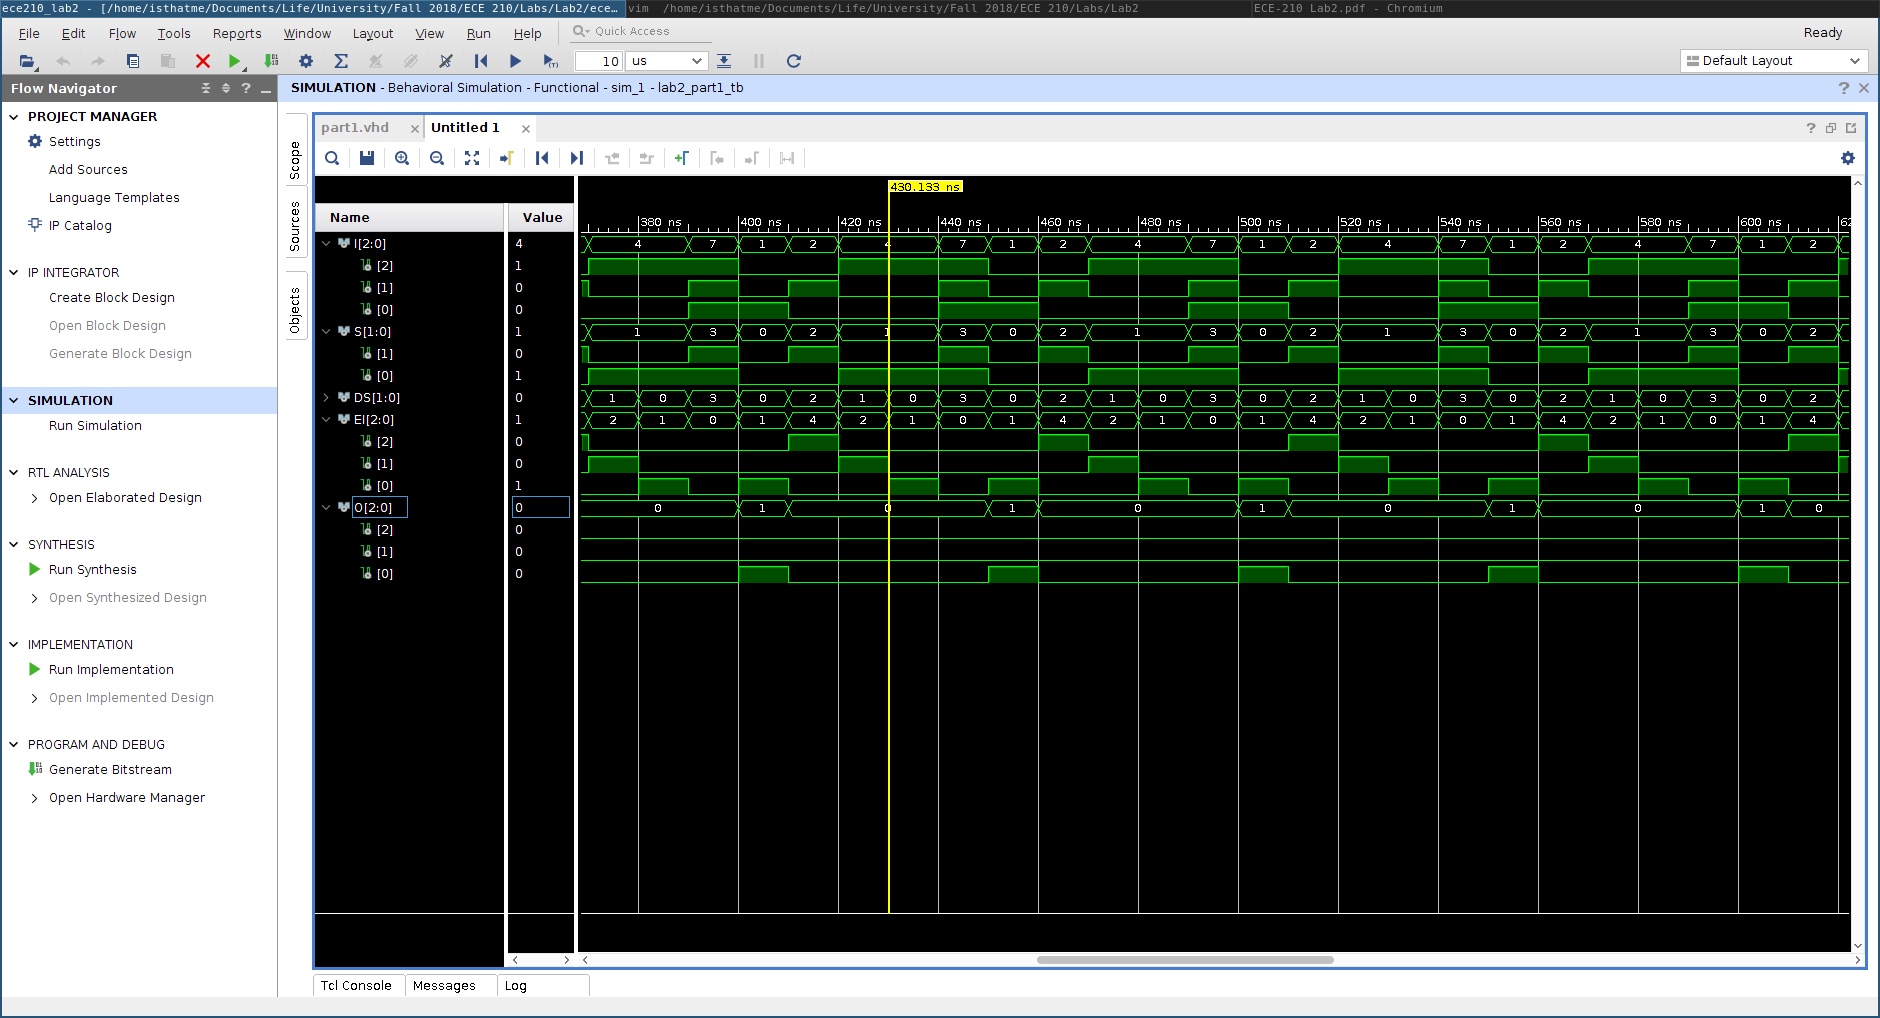
\includegraphics[width=\linewidth]{MUX_DEMUX.png}
        \caption{Results from Multiplexer/Demultiplexer circuit simulation in Xilinx Vivado}
        \label{fig:part1_sim}
    \end{figure}

    \paragraph{Part 2}
    The VHDL design was able to correctly control the lab access and alarm signals
    as specified, both in the simulated results and the tests on the physical board.
    Below are images of the simulation waveform and a physical test of one of the
    input combinations.

    \begin{figure}[H]
        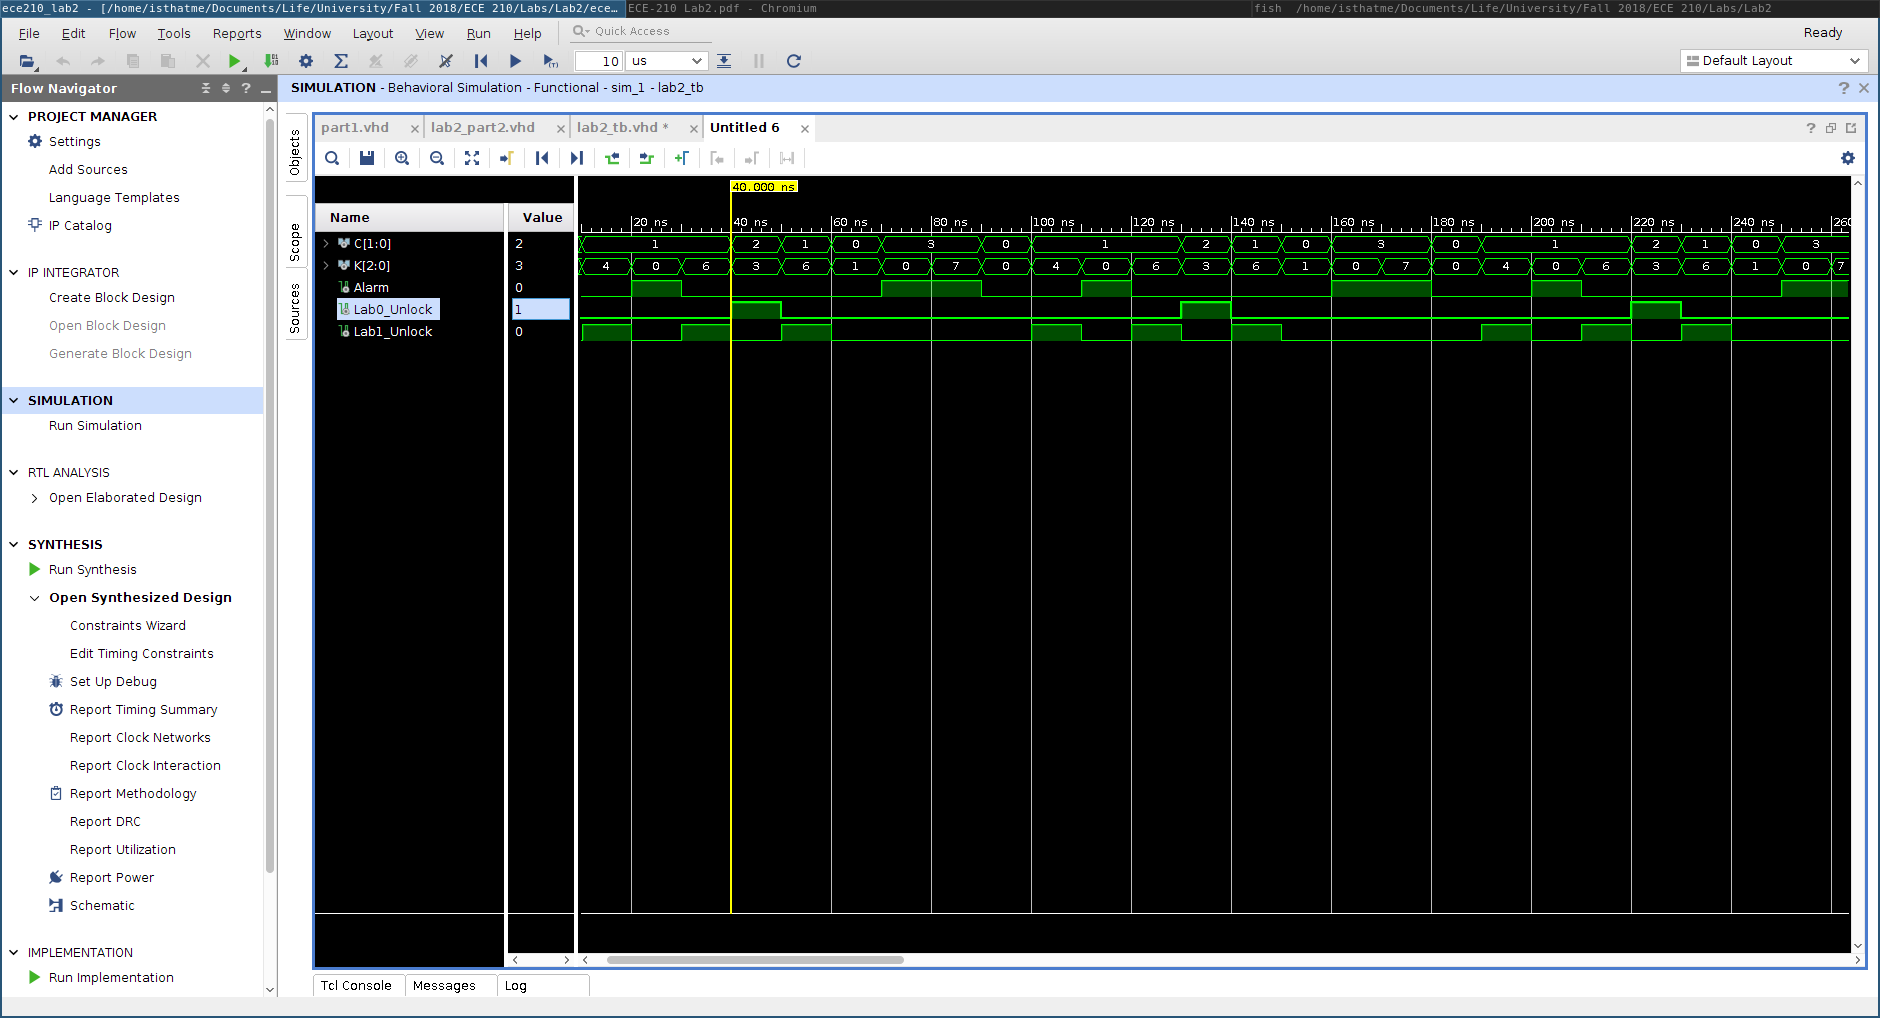
\includegraphics[width=\linewidth]{Access_control.png}
        \caption{Results from Lab Access Control circuit simulation in Xilinx Vivado}
        \label{fig:part2_sim}
    \end{figure}

    \begin{figure}[H]
        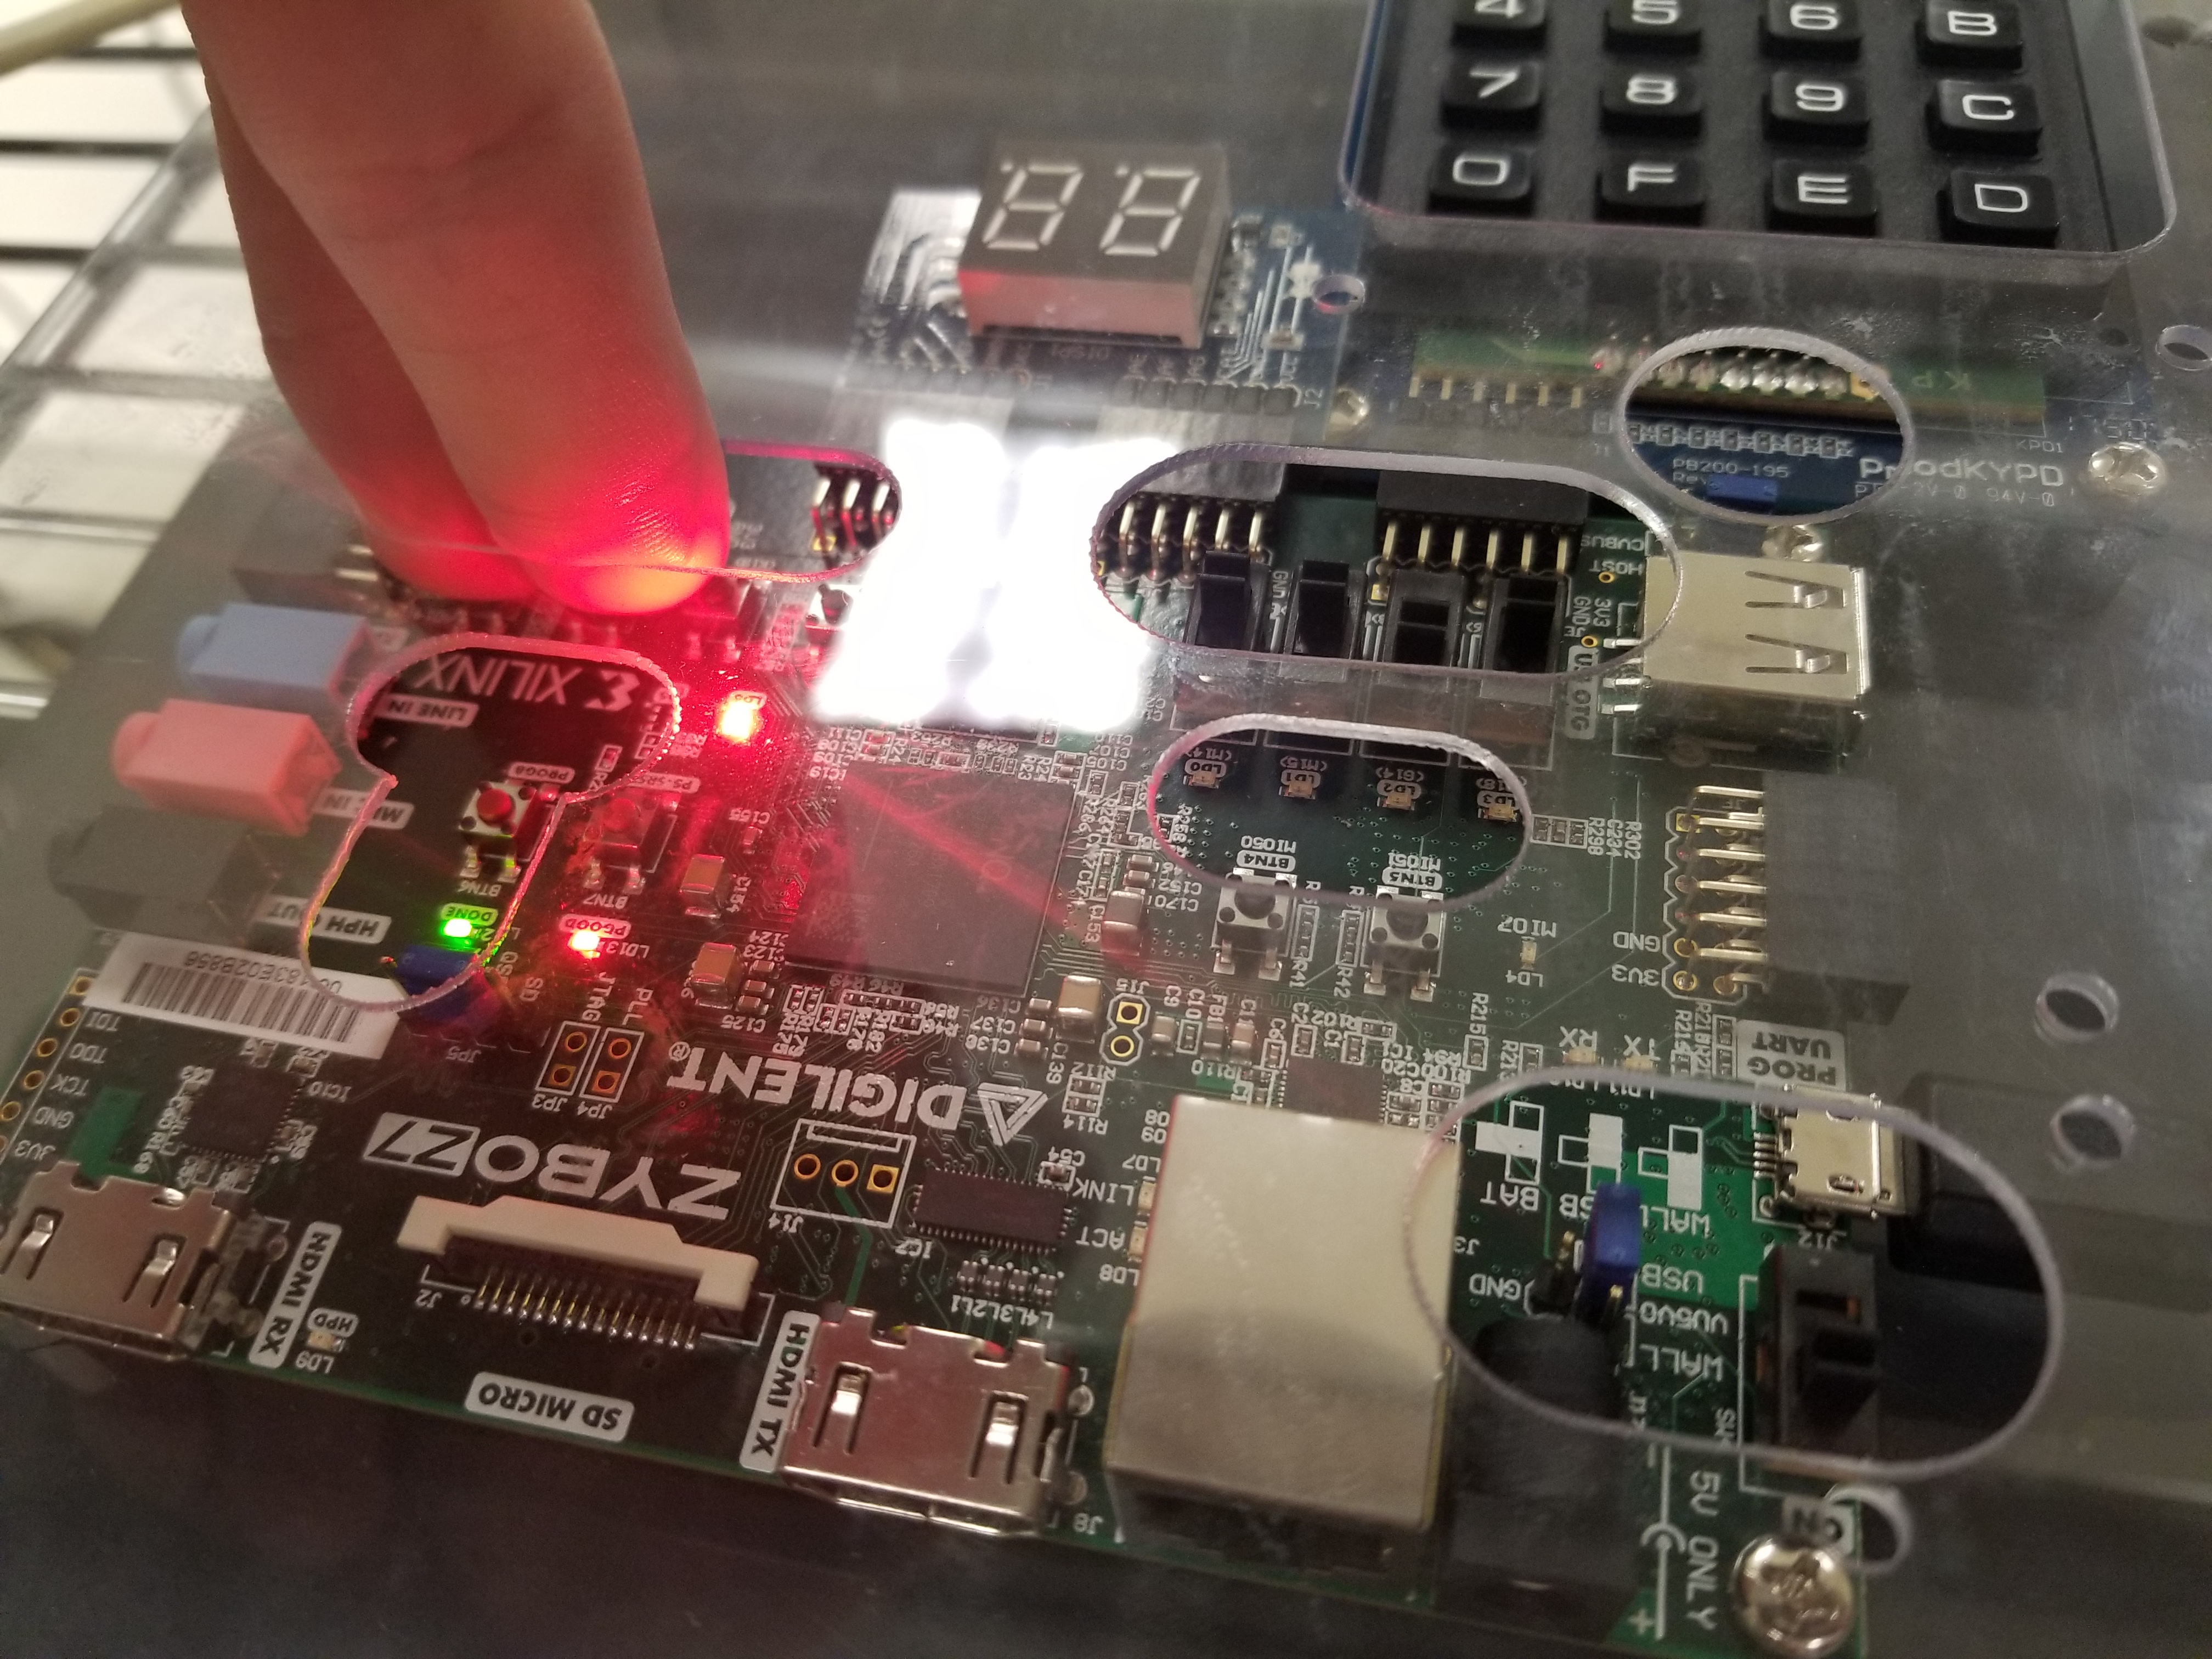
\includegraphics[width=\linewidth]{access_testing.jpg}
        \caption{Physically Testing the Lab Access Control system on an FPGA board}
        \label{fig:part2_testing}
    \end{figure}


    \section{Discussion}
    Multiplexing and demultiplexing circuits are designed using 'selection' elements.
    These elements can also be repurposed to create functional
    and practical circuits for real life applications.
    
    \paragraph{Mux and Demux Circuit}

    \begin{enumerate}
            \item When the mux and demux select signals are in an unused state,
                There will be no signal outputs going to any of the engineers.
                
            \item Waveform can be found in the results section.

            \item The advantage of ICs is that you can physically see the layout of the circuit. As well, you can probe the internal connections.
                However, it is quite tedious to connect a large number of ICs together,
                and it can be quite error prone.
                The advantages of using an FPGA is that you can get a computer to make the connections for you.
                This allows you to rapidly design and prototype circuits. However, a disadvantage is that
                you cannot physically inspect the circuit and probe the internals.
    \end{enumerate}

    \paragraph{Lab Access Control}

    \begin{enumerate}
            \item The simulation waveform is provided above in the results section.

            \item I would rate the system as somewhat effective. However, it is not at all upgradable or expandable as designed.
                There are too few possible combinations, and these are set on toggle switches, which is not
                secure.
                It performs according to the given specifications.

            \item Something with a momentary keypad, as well as a programmable access control system.
                This would allow access to be given and revoked, passwords to be longer, and easily changable
                combinations.

    \end{enumerate}


    \section{Conclusion}
    It is sometimes necessary in real-life applications to use the fundamental elements
    of circuit technology to implement boolean expressions in hardware, when such
    hardware may be unavailable. Even if these packages may be purchased from a
    manufacturer, sometimes a situation may call for an implementation that cannot
    use these elements.
    Also, FPGAs are useful tools for the quick design and development of functional circuits.
    These circuits can borrow ideas and methods of operation from each other to more
    efficiently and creatively implement the desired functionality.

\end{document}

